\section{Encoding a Change Log}

The change log used in the following section was generated using data from The Paragenetic Mode for Copper Minerals database \cite{Morrison2016}.
The change logs were marked up in HTML to facilitate RDFa or JSON-LD.
Figure \ref{changelog_zoomed} shows the visible text of the mineral Abswurmbachite in the change log.
\begin{figure}[b]
	\centering
	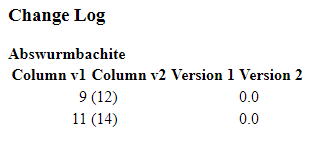
\includegraphics[scale=0.80]{Changelog-zoomed.png}
	\caption{Abswurmbachite entry in the Copper Dataset change log.}
	\label{changelog_zoomed}
\end{figure}
Notice how the column indexes do not match across versions due to additions and invalidations of columns.
The versioning model forms a conceptual mapping based on attributes, not on tabular indexes.
The change logs follow a common format with three sections: Additions, Invalidations, and then Modifications.
The sections may be further grouped by column or row additions.
The division means that changes are not published into the change log as they are found, but instead organized and grouped beforehand.

\subsection{Resource Description Framework in Attributes}

Very little natural language is used in the change log to regularize the format and improve compatibility with RDFa.
Listing \ref{rdfa_list} shows the text necessary to lay out the first four lines of Figure \ref{changelog_zoomed}.
\begin{listing}
	\begin{minted}[linenos, frame=lines, framesep=2mm, breaklines]{HTML}
<h3>Change Log</h3>
  <div about="Version1" rel="vo:hasAttribute">
    <div resource="v2:Abswurmbachite" typeof="vo:Attribute">
      <span style="font-weight:bold" property="http://www.w3.org/2000/01/rdf-schema#label">Abswurmbachite</span>
      <table rel="vo:Undergoes">
        <tr  about="ChangeAbswurmbachite12" typeof="vo:Change">
          <td align="right" rev="vo:Undergoes" resource="v1:AttributeAbswurmbachite12v1" typeof="vo:Attribute"> 9</td>
          <td property="vo:resultsIn" resource="v2:AttributeAbswurmbachite12v2" typeof="vo:Attribute">(12)</td>
          <td>          </td>
          <td>       0.0</td>
          <span about="Version1" property="vo:hasAttribute" resource="v1:AttributeAbswurmbachite12v1"></span>
          <span about="Version2" property="vo:hasAttribute" resource="v2:AttributeAbswurmbachite12v2"></span>
        </tr>
      </table></div></div><br>
	\end{minted}
	\caption{Abswurmbachite RDFa.\label{rdfa_list}}
\end{listing}
While the content only shows four lines, the underlying markup takes up three and a half times as many lines.
Line 2 of Listing \ref{rdfa_list} states that all following resources will be attributes of Version 1.
Line 3 defines such an attribute.
Lines 5 through 8 define the changes Abswurmbachite undergoes.
Because RDFa embeds the statements within the content, the triples appear along with the described text.
Lines 11 and 12 define complete triples which do not appear in the visible document.
The lines complete the graph, but must be included in HTML span tags because RDFa only allows a single triple within each tag.
Notice that the RDFa encoding does not interact with any of the visible content, but still relies on the tag structure to properly link concepts together.
The resulting markup is completely constrained by RDFa's adherence to the visible content but does not leverage the benefits of RDFa's ability to incorporate the visible content.

\subsection{JavaScript Object Notation for Linked Data}
After encountering the limitations of using RDFa to include the versioning ontology into the change log, JSON-LD was used.
The JSON data is independent of the visible content's structure in the change log.
Listing \ref{json_list} provides the alternative encoding of the Abswurmbachite entry using JSON-LD.
The entry is significantly longer, almost three times longer than the RDFa entry and ten times longer than the original visible content.
Instead of including the data for each entry at the beginning or end of the document, each change block is separated into the particular \textit{div} section for that change.
This choice allows consumers to extract pertinent change information without needing to ingest the entire log.

The change logs created with RDFa or JSON-LD demonstrate progress towards documents which are both human and machine-readable.
The implementation provides evidence that JSON-LD is better suited to embed a versioning graph into a change log than RDFa.
RDFa suffers limitations since it is constrained by the content's structure.
Notice the merged row and column identifiers in the \mintinline{html}{resource} attribute of lines 7 and 8 in Listing \ref{rdfa_list}.
The row identifier, Abswurmbachite, and column identifier, 12, were merged because the tag could only support a single value.
The merged attribute stems from a mismatch between the model's structure, the order in which data appears in the change log, and the way RDFa links properties together.
Because the row label forms the outermost encapsulation, data in the tag cannot instantiate both row identifiers and implicitly link the identifiers separately.
To do so would require explicitly instantiating the attribute in a non-visible part of the document, defeating the purpose of using RDFa to implicitly encode the versioning graph into the document.
%\begin{listing}
\begin{mdframed}[topline=false, bottomline=false, leftline=false, rightline=false]
	\begin{minted}[linenos, frame=lines, breaklines]{HTML}
<h3>Change Log</h3>
  <div about="v1:Abswurmbachite">
    <span style="font-weight:bold" property="http://www.w3.org/2000/01/rdf-schema#label">Abswurmbachite</span>
    <table>
    <tr  id="ModifyChangeAbswurmbachite12">
      <td align="right"> 9</td>
      <td >(12)</td>
      <td>          </td>
      <td>       0.0</td>
      <script type="application/ld+json">
[
  {
    "@context": "https://orion.tw.rpi.edu/~blee/provdist/GCMD/VO.jsonld", 
    "@id": "http://CUdb.com/v1/AttributeAbswurmbachite9", 
    "@reverse": {
      "hasAttribute": "Version1"
    }, 
    "@type": "vo:Attribute", 
    "label": "Primary", 
    "undergoes": "http://orion.tw.rpi.edu/~blee/provdist/CU/DTDI/CUjsonlog.html#ModifyChangeAbswurmbachite12"
  }, 
  {
    "@context": "https://orion.tw.rpi.edu/~blee/provdist/GCMD/VO.jsonld", 
    "@id": "http://orion.tw.rpi.edu/~blee/provdist/CU/DTDI/CUjsonlog.html#ModifyChangeAbswurmbachite12", 
    "@type": "vo:ModifyChange", 
    "resultsIn": "http://CUdb.com/v2/AttributeAbswurmbachite12"
  }, 
  {
    "@context": "https://orion.tw.rpi.edu/~blee/provdist/GCMD/VO.jsonld", 
    "@id": "http://CUdb.com/v2/AttributeAbswurmbachite12", 
    "@reverse": {
      "hasAttribute": "Version2"
    }, 
    "@type": "vo:Attribute", 
    "label": "Primary"
  }
]
      </script></tr></table></div><br>
	\end{minted}
	
	%	\caption{Abswurmbachite JSON-LD\label{json_list}}
	%\end{listing}
	\captionof{listing}{Abswurmbachite JSON-LD.\label{json_list}}
\end{mdframed}

Both structured data implementations break up the graph across attributes so that individual parts of the graph can be extracted.
The practice of a one-node JSON object is generally helpful for many web applications to load data quickly, but since the change log is not an application, it makes more sense to break up the content.
Changes to individual attributes can be identified using anchors on the web page, then agents need only extract and parse the linked data to the attributes' specific entries.
This way, a subgraph of only the pertinent attributes can be created without first ingesting the entire versioning graph.